\section{Prospetto economico}
In questa sezione vengono presentate, per ciascun periodo del progetto\ped{G}, le ore di impegno calcolate a preventivo\ped{G} per i ruoli coinvolti, divise tra ore di investimento\ped{G} e ore contabilizzate. Si ricorda che il periodo di \textit{Analisi dei Requisiti\ped{G}} non è a carico del committente\ped{G} e quindi non sarà considerata nel calcolo del preventivo\ped{G}, ma solo indicate come risorse di investimento\ped{G}.
\subsection{Analisi dei Requisiti}
Nel priodo riguardante la fase di \textbf{Analisi dei Requisiti\ped{G}} le ore tra i ruoli sono state divise nel seguente modo:

\begin{table}[H]
	\begin{center}
		\begin{tabular}{|l|c|c|}
			\hline
			\textbf{Ruolo}	& \textbf{Ore} & \textbf{Costo} \\
			\hline
			Responsabile	&	43	&	 1290	\\
			\hline
			Amministratore	&	18	&	 360	\\
			\hline
			Analista		&	84	&	 2100	\\
			\hline
			Verificatore	&	65	&	 975	\\
			\hline
			\textbf{Totale} &	210	&	4725	\\
			\hline
		\end{tabular}
	\end{center}
	\caption{Costo per ruolo, Analisi dei Requisiti}
\end{table}

\begin{figure}[H]
	\centering
	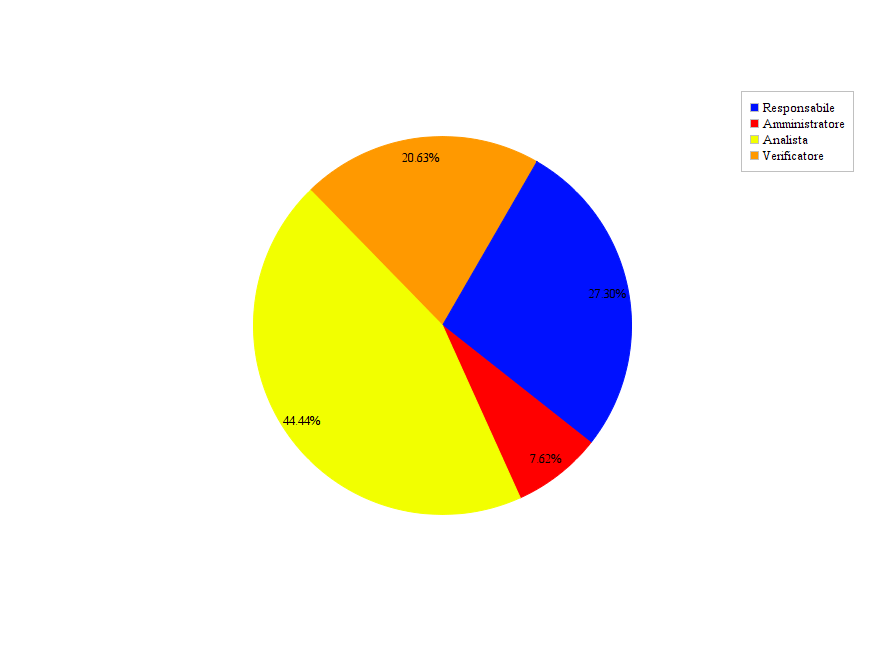
\includegraphics[scale=0.4]{immagini/Grafi/CostoAR}
	\caption{Costo per ruolo, Analisi dei Requisiti}
\end{figure}

\subsection{Progettazione Architetturale}
Nel periodo riguardante la \textbf{Progettazione Architetturale\ped{G}} le ore tra i ruoli sono state divise nel seguente modo:

\begin{table}[H]
	\begin{center}
		\begin{tabular}{|l|c|c|}
			\hline
			\textbf{Ruolo}	& \textbf{Ore} &	\textbf{Costo}	 \\
			\hline
			Responsabile	&	6	&	180		\\
			\hline
			Amministratore	&	8	&	160		\\
			\hline
			Progettista		&	141	&	3102	\\
			\hline
			Verificatore	&	70	&	1050	\\
			\hline
			\textbf{Totale}	&	225	&	4492	\\
			\hline
		\end{tabular}
	\end{center}
	\caption{Costo per ruolo, Progettazione Architetturale}
\end{table}

\begin{figure}[H]
	\centering
	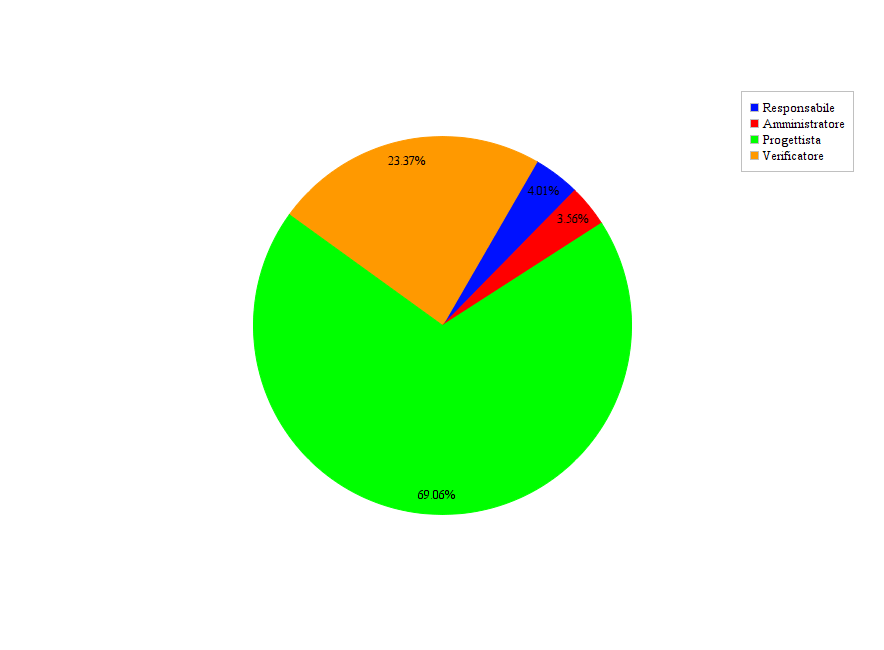
\includegraphics[scale=0.4]{immagini/Grafi/CostoPA}
	\caption{Costo per ruolo, Progettazione Architetturale}
\end{figure}

\subsection{Progettazione di Dettaglio}
Nel periodo riguardante la \textbf{Progettazione di Dettaglio\ped{G}} le ore tra i ruoli sono state divise nel seguente modo:

\begin{table}[H]
	\begin{center}
		\begin{tabular}{|l|c|c|}
			\hline
			\textbf{Ruolo}	& \textbf{Ore} &	\textbf{Costo}	 \\
			\hline
			Responsabile	&	7	&	210		\\
			\hline
			Amministratore	&	5	&	100		\\
			\hline
			Progettista		&	86	&	1892	\\
			\hline
			Verificatore	&	42	&	630		\\
			\hline
			\textbf{Totale}	&	140	&	2832	\\
			\hline
		\end{tabular}
	\end{center}
	\caption{Costo per ruolo, Progettazione di Dettaglio}
\end{table}

\begin{figure}[H]
	\centering
	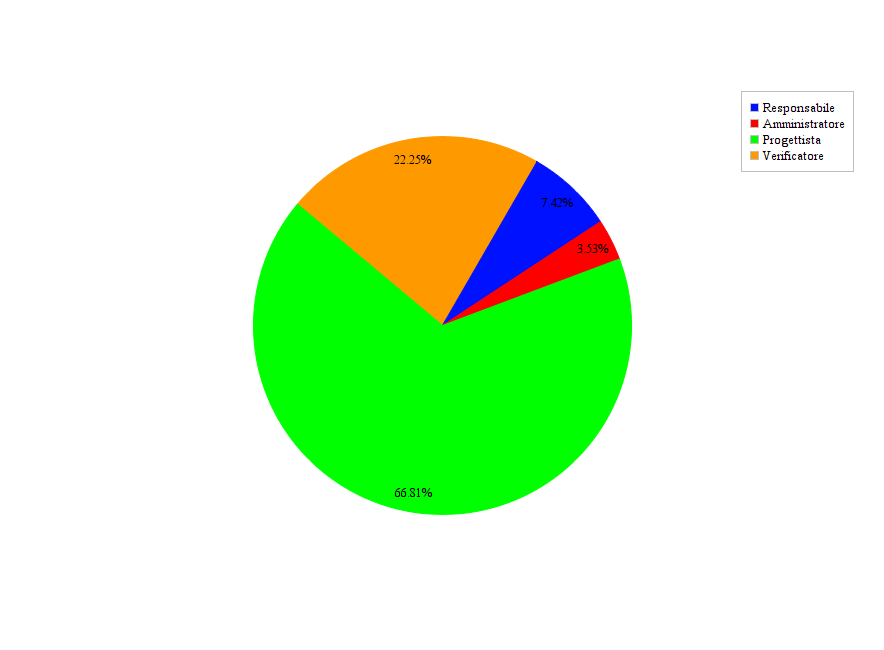
\includegraphics[scale=0.4]{immagini/Grafi/CostoPD}
	\caption{Costo per ruolo, Progettazione di Dettaglio}
\end{figure}


\subsection{Codifica}
Nel periodo riguardante la \textbf{Codifica\ped{G}} le ore tra i ruoli sono state divise nel seguente modo:

\begin{table}[H]
	\begin{center}
		\begin{tabular}{|l|c|c|}
			\hline
			\textbf{Ruolo}	& \textbf{Ore} &	\textbf{Costo}	 \\
			\hline
			Responsabile	&	11	&	330		\\
			\hline
			Amministratore	&	4	&	80		\\
			\hline
			Progettista		&	25	&	550		\\
			\hline
			Programmatore	&	133	&	1995	\\
			\hline
			Verificatore	&	75	&	1125	\\
			\hline
			\textbf{Totale}	&	248	&	4080	\\
			\hline
		\end{tabular}
	\end{center}
	\caption{Costo per ruolo, Codifica}
\end{table}

\begin{figure}[H]
	\centering
	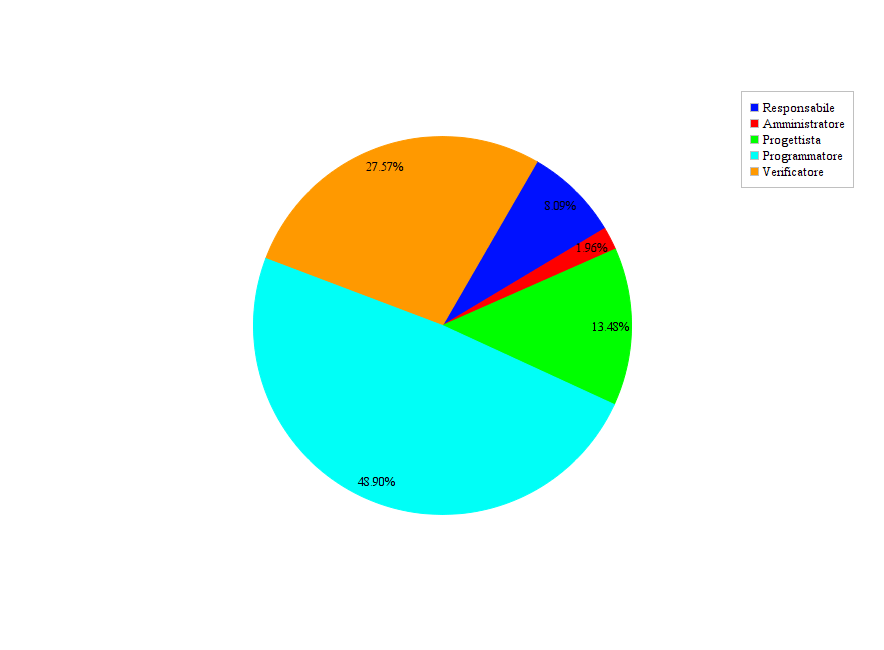
\includegraphics[scale=0.4]{immagini/Grafi/CostoCod}
	\caption{Costo per ruolo, Codifica}
\end{figure}

\subsection{Verifica e Validazione}
Nel periodo riguardante la \textbf{Verifica e Validazione\ped{G}} le ore tra i ruoli sono state divise nel seguente modo:

\begin{table}[H]
	\begin{center}
		\begin{tabular}{|l|c|c|}
			\hline
			\textbf{Ruolo}	& \textbf{Ore} &	\textbf{Costo}	 \\
			\hline
			Responsabile	&	9	&	270		\\
			\hline
			Progettista		&	20	&	440		\\
			\hline
			Verificatore	&	93	&	1395	\\
			\hline
			\textbf{Totale}	&	122	&	2105	\\
			\hline
		\end{tabular}
	\end{center}
	\caption{Costo per ruolo, Verifica e Validazione}
\end{table}

\begin{figure}[H]
	\centering
	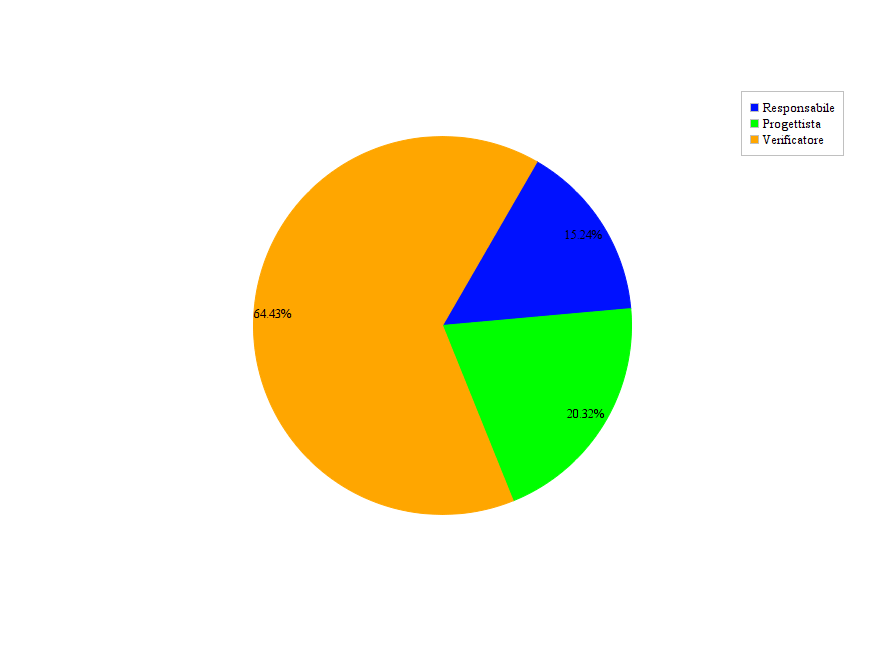
\includegraphics[scale=0.4]{immagini/Grafi/CostoVV}
	\caption{Costo per ruolo, Verifica e Validazione}
\end{figure}

\subsection{Totale}
\subsubsection{Ore totali}
Le ore totali, previste per la realizzazione dell'intero progetto\ped{G}, comprese le ore di investimento\ped{G}, sono riportate nella tabella seguente.

\begin{table}[H]
	\begin{center}
		\begin{tabular}{|l|c|c|c|}
			\hline
			\textbf{Ruolo}	& \textbf{Ore} &	\textbf{Ore remunerabili}	 &\textbf{Costo} \\
			\hline
			Responsabile	&	76	&	33	&	990	\\
			\hline
			Amministratore	&	35	&	17	&	340	\\
			\hline
			Analista		&	84	&	0	&	0	\\
			\hline
			Progettista		&	272	&	272	&	5984	\\
			\hline
			Programmatore	&	133	&	133	&	1995	\\
			\hline
			Verificatore	&	345	&	280	&	4200	\\
			\hline
			\textbf{Totale}	&	945	&	735	&	13509	\\
			\hline
		\end{tabular}
	\end{center}
	\caption{Costo totale per ruolo}
\end{table}

\begin{figure}[H]
	\centering
	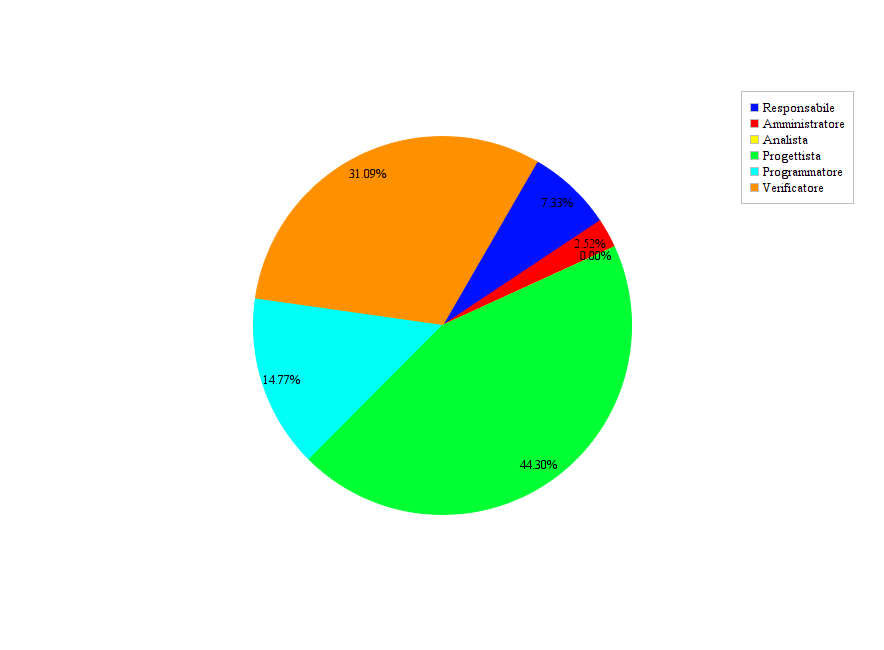
\includegraphics[scale=0.4]{immagini/Grafi/CostoTot}
	\caption{Costo per ruolo, Costo Totale}
\end{figure}

\subsubsection{Conclusioni}
<<<<<<< HEAD
Il costo totale del progetto\ped{G}, indicato nella tabella 18, viene arrotondato a \textbf{€ 13500}.\\
=======
Il costo totale del progetto, indicato nella tabella 18, viene arrotondato a \textbf{€ 13500}.\\
>>>>>>> origin/master
